% CPU/GPU correlation
GPUs are usually used in a heterogeneous model containing two different processors, namely the CPU and the GPU as presented on \cref{fig:hw-cpu-gpu}.
The configuration of this CPU/GPU architecture comes in different varieties, however, the variant with one CPU communicating with one GPU is the most common.
In addition there exists configurations such as integrated GPUs for laptops where the CPU and GPU uses one shared memory block.
As well configurations containing a multiple amount of GPUs for more demanding computational work.

\begin{figure}[ht]
	\centering
	\fbox{
		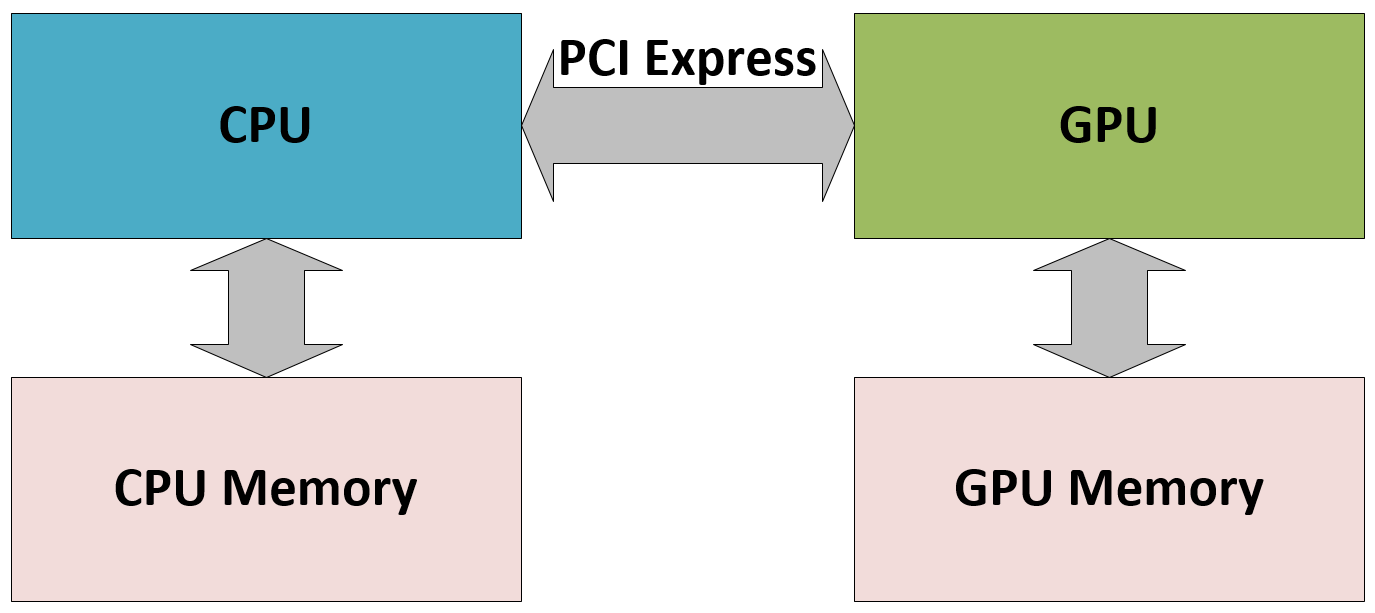
\includegraphics[width=0.8\textwidth]{figs/hw/hw-cpu-gpu}}
	\caption{CPU/GPU architecture}
	\label{fig:hw-cpu-gpu}
\end{figure}

The communication between the CPU and GPU serves multiple purposes, which is key part in realizing both the graphical and computational work of the GPU.
Further information regarding this programming model is presented in \cref{ch-programming-model}, instead this section concentrates on how this communication is handled out.

Older generation CPUs depended on the chipset located on the motherboard to communicate with GPUs as well as other outside components such as memory, I/Os and so on.
However, this made the processors performance highly dependent on the chipset, as communication between RAM and GPUs went through the \textit{northbridge} part of the chipset.
To avoid this dependency the implementation of the northbridge and the remaining chipset functionalities were moved to the CPUs itself, improving the performance.

Thereby the communication between the CPU and GPU is highly dependent on the CPU itself, and the bus used between these two processors, namely the PCI Express bus.


%TODO Add more? SLI https://en.wikipedia.org/wiki/Scalable_Link_Interface






